% !TEX root = main.tex
\onecolumn
\newpage


%\begin{titlepage}
  \begin{centering}
    \vspace*{1cm}
    
    \textbf{\Large Supporting Information}\\
    \vspace{0.5cm}
    \textbf{\Large \linearpartition: Linear-Time Approximation of RNA Folding Partition Function and Base Pairing Probabilities}\\
    \vspace{0.5cm}
    \textbf{\large
    He Zhang, Liang Zhang, David H.~Mathews and Liang Huang}
    \vspace{1.5cm}
    
  \end{centering}
%\end{titlepage}

\setcounter{figure}{0}
\renewcommand{\thefigure}{SI\,\arabic{figure}} % spacing
\setcounter{table}{0}
\renewcommand{\thetable}{SI\,\arabic{table}}
\setcounter{page}{1}
% \renewcommand{\thepage}{\arabic{chapter}.\arabic{page}} 

\setcounter{section}{0}
\renewcommand\thesection{\Alph{section}}
\setcounter{subsection}{0}
\renewcommand\thesubsection{\Alph{section}.\arabic{subsection}}

% \setcounter{reference}{0}


\section{Details of the Efficient Implementation}
\label{sec:si:algdetails}

\titleformat{\subsection}%[runin]
{\normalfont\bfseries}% formatting commands to apply to the whole heading
        {\thesubsection}% the label and number
        {0.5em}% space between label/number and subsection title
        {#1}% formatting commands applied just to subsection title
        []
        
\subsection{Data Structures}

%\begin{table}
In the main text, for simplicity of presentation, $Q$ is described as a hash from span $[i,j]$
to $\Qf{i}{j}$, but in our actual implementation,
to make sure the overall runtime is $O(n b^2)$,  we implement $Q$ as
an array of $n$ hashes, where each $Q[j]$ is a hash
mapping $i$ to $Q[j][i]$ which is conveniently notated as \Qf{i}{j} in the main text. It is important to note that the first dimension $j$ is the right boundary
and the second dimension $i$ is the left boundary of the span $[i,j]$. See the following table for a summary of notations and the corresponding actual implementations.
Here we use Python notation for simplicity, but in actual system we implement with C++.
\begin{center}
%\resizebox{0.5\textwidth}{!}{
\begin{tabular}{l|l}
notations in this paper & Python implementation\\
\hline
%$Q\gets$ hash() & \verb|Q = defaultdict(lambda : defaultdict(float))|\\
$Q\gets$ hash() & {\tt Q = [defaultdict(float) \textbf{for} \_ \textbf{in} range(n)]}\\
\Qf{i}{j} & \verb|Q[j][i]| \\
$[i,j]$ in $Q$ & {\tt i \textbf{in} Q[j]}\\
{\bf for each} $i$ such that $[i,j]$ in $Q$ & {\tt \textbf{for} i \textbf{in} Q[j]}\\
{\bf delete} $[i,j]$ from $Q$ & {\tt \textbf{del} Q[j][i]}
\end{tabular}
%}
\end{center}
%\end{table}

\subsection{Complexity Analysis}

In the partition function calculation (inside phase) in Fig.~\ref{fig:algorithm},
the number of states is $O(nb)$ because each $Q[j]$ contains at most $b$ states (\Qf{i}{j}'s) after pruning. Therefore the space complexity is $O(nb)$.
For time complexity, there are three nested loops, the first one ($j$) with $n$ iterations,
the second ($i$) and the third ($k$) loops both have $O(b)$ iterations thanks to pruning, so the overall runtime is $O(nb^2)$.

\subsection{Outside Partition Function and Base Pairing Probability Calculation}
\label{sec:outside}

After we compute the partition functions \Qf{i}{j} on each span $[i,j]$ (known as the ``inside partition function''),
we also need to compute the complementary function \Qhatf{i}{j} for each span known as
the ``outside partition function'' in order to derive the base-pairing probabilities. 
Unlike the inside phase, this outside partition function is calculated from top down,
with $\Qhatf{1}{n} = 1$ as the base case.
\begin{equation*}
\begin{split}
\Qhatf{i}{j} & = \Qhatf{i}{j+1} \cdot e^{-\frac{\delta(\vecx, j+1)}{RT}} \\
                  & + \sum_{k < i} \Qhatf{k}{j+1} \cdot \Qf{k}{i-2} \cdot e^{-\frac{\xi(\vecx,i-1,j+1)}{RT}} \\
                  & + \sum_{k > j+1} \Qhatf{i}{k} \cdot \Qf{j+2}{k-1} \cdot e^{-\frac{\xi(\vecx,j+1,k)}{RT}}
\end{split}
\end{equation*}
Note that the second line is only possible when $x_{i-1} x_{j+1}$ can form a base pair
(otherwise $e^{-\frac{\xi(\vecx,i-1,j+1)}{RT}} = 0$)
and the third line has a constraint that $x_{j+1}x_k$ can form a base pair 
(otherwise $e^{-\frac{\xi(\vecx,j+1,k)}{RT}} = 0$).


For each $(i,j)$  where $x_i x_j$ can form a base pair, we compute its pairing probability:
\[
p_{i,j}  = \sum_{k \leq i} \Qhatf{k}{j} \cdot \Qf{k}{i-1} \cdot e^{-\frac{\xi(\vecx,i,j)}{RT}} \cdot \Qf{i+1}{j-1}
\]

The whole ``outside'' computation takes $O(n^3)$ without pruning,
but also $O(nb^2)$ with beam pruning.
See Fig.~\ref{fig:outside} for the pseudocode to compute the outside partition function and base pairing probabilities.

%\subsection{Supporting Pseudocode}

\section{Details of datasets, baselines and methods}

% \newpage
\subsection{Datasets}
\label{sec:datasets}

We use sequences from two datasets, ArchiveII and RNAcentral.
The archiveII dataset 
(available in \url{http://rna.urmc.rochester.edu/pub/archiveII.tar.gz}) is % \cite{sloma+mathews:2016}, 
a diverse set with 3,857 RNA sequences and their secondary structures.
It is first curated in the 1990s to contain sequences with structures that were well-determined by comparative sequence analysis~\cite{mathews+:1999}% [72] 
and updated later with additional structures~\cite{sloma+mathews:2016}. % [96].  
% and is available in \url{http://rna.urmc.rochester.edu/pub/archiveII.tar.gz}.
We remove 957 sequences that appear both in the ArchiveII and the S-Processed datasets~\cite{Andronescu+:2007}, 
because CONTRAfold uses S-Processed for training. 
We also remove all 11 Group II Intron sequences 
because there are so few instances of these that are available electronically.
Additionally, we removed 30 sequences in the tmRNA family because the annotated structure for each of these sequences contains fewer than 4 pseudoknots, 
which suggests the structures are incomplete. 
These preprocessing steps lead to a subset of ArchiveII with 2,859 reliable secondary structure 
% RNA sequence and structure pairs 
examples 
distributed in 9 families. 
See~\ref{tab:archiveII} for the statistics of the sequences we use in the ArchiveII dataset.
% But since CONTRAfold (v2.02) machine-learned model is trained on the S-Processed dataset \cite{},
% we removed those overlap sequences. 
% As in \linearfold paper, we also remove those sequences CONTRAfold (v2.02) used for training.
% The remaining dataset contains 2889 RNA sequences from 9 families, 
% with average length 222 $nt$ and max length 2968 $nt$.
Moreover, we randomly sampled 22 longer RNA sequences (without known structures) from RNAcentral~\cite{rnacentral:2017} 
% (The RNAcentral Consortium, 2017) 
(\url{https://rnacentral.org/}),
with sequence lengths ranging from 3,048~{\it nt} to 244,296~{\it nt}.
For the sampling, we evenly split the range from $3,000$ to $244,296$ (the longest) into 24 bins by log-scale, and for each bin we
randomly select a sequence (there are bins with
no sequences).
% (Homo Sapiens Transcript NONHSAT168677.1, from the NONCODE database (Zhao et al., 2016)).
% We run all experiments 
% % (compiled by GCC 4.9.0) 
% on a Linux machine, 
% with 2.90GHz Intel Core i9-7920X CPU and 64G memory.

To show the approximation quality on random RNA sequences, 
we generated 30 sequences with uniform distribution over \{A, C, G, U\}.
% The lengths of these sequences are 100, 200, ..., 3000.
The lengths of these sequences are spaced in 100 nucleotide intervals from 100 to 3,000.
% with lengths range from 100~{\it nt} to 3,000~{\it nt}. 


\begin{table}[!h] % hzhang: redo with new data
  \centering
  \large
  \setlength{\tabcolsep}{12pt}
  \begin{tabular}{r|rr|rrr}
    & \multicolumn{2}{c|}{\# of seqs} & \multicolumn{3}{c}{length} \\
    Family & total & used & avg & max & min \\
    \hline
    tRNA  & 557 & 74  & 77.3  & 88 &58  \\
    5S rRNA & 1,283 & 1,125 & 118.8 & 135 &102  \\
    SRP RNA & 928 & 886 & 186.1 & 533 & 28\\
    RNase P RNA & 454 & 182 & 344.1 & 486 & 120 \\
    tmRNA & 462 & 432 & 369.1 & 433 & 307 \\
    Group I Intron  & 98  & 96  & 424.9 & 736 &210  \\
    Group II Intron  & 11  & 0  & - & -&-  \\
    telomerase RNA  & 37  & 37  & 444.6 & 559 &382\\
    16S rRNA  & 22  & 22  & 1,547.9  & 1995 & 950\\
    23S rRNA  & 5 & 5 & 2,927.4  & 2968& 2904\\
    \hline
    {\em Overall} & 3,846 & 2,859 & 221.1 &2968 &28 \\
  \end{tabular}
  \\[0.3cm]
  % \smallskip
  \caption{Statistics of the sequences in the ArchiveII dataset used in this work.
    \label{tab:archiveII}}
\end{table}


\subsection{Baseline Software}

We use two baseline software packages: 
(1) \viennarnafold %~\cite{lorenz+:2011}
(Version 2.4.11) 
from 
\url{https://www.tbi.univie.ac.at/RNA/download/sourcecode/2_ 4_x/ViennaRNA-2.4.11.tar.gz} 
and 
(2) \contrafold %~\cite{do+:2006}
(Version 2.0.2) 
from
\url{http://contra.stanford.edu/}.
\viennarnafold is a widely-used RNA structure prediction package,
while \contrafold is a successful machine learning-based RNA structure prediction system.
Both provide partition function and base pairing probability calculations based on 
the classical cubic runtime algorithm.
Our comparisons mainly focus on the systems with the same model, 
i.e., \linearpartitionv vs. \viennarnafold and \linearpartitionc vs. \contrafold.
In this way the differences are based on algorithms themselves rather than models.
% bugs in contrafold
We found a bug in \contrafold by comparing our results to CONTRAfold, 
which led to overcounting multiloops in the partition function calculation.
We corrected the bug, and all experiments are based on this bug-fixed version of \contrafold.


\subsection{Evaluation Metrics and Significance Test}

Due to the uncertainty of base-pair matches existing in comparative analysis
and the fact that there is fluctuation in base pairing at equilibrium,
we consider a base pair to be correctly predicted if it is also displaced by one
nucleotide on a strand~\cite{mathews+:1999}.
Generally, if a pair $(i,j)$ is in the predicted structure, we consider it a
correct prediction if one of $(i,j)$, $(i-1,j)$, $(i+1,j)$, $(i,j-1)$, $(i,j+1)$ is in the
ground truth structure.
% We also report the accuracy using exact base pair matching instead of this
% method, in Figure~\ref{tab:accuracy_nos}. 
%To evaluate the accuracy, 
% Both sensitivity and PPV are reported.
%Positive Predictive Value
%(PPV), 

We use Positive Predictive Value (PPV)
and sensitivity 
as accuracy measurements. 
Formally, denote $\vecy$ as the predicted structure and $\vecy^{*}$ as the ground
truth, we have:
% $\ppv = \frac{\text{true positives}}{\text{true positives} +
%   \text{false positives}} = \frac{|\vecy \cap \vecy^*|}{|\vecy|} $
% $ \sens = \frac{\text{true positives}}{\text{true positives} +
%   \text{false negatives}} =
% \frac{|\vecy \cap \vecy^*|}{|\vecy^*|}$

$$\ppv = \frac{\#_{\text {TP}}}{\#_{\text {TP}} + \#_{\text {FP}}}  = 
\frac{|\pairs(\vecy) \cap \pairs(\vecy^*)|}{|\pairs(\vecy)|} $$

$$ \sens = \frac{\#_{\text {TP}}}{\#_{\text {TP}} + \#_{\text {FN}}}  =
\frac{|\pairs(\vecy) \cap \pairs(\vecy^*)|}{|\pairs(\vecy^*)|}$$
where $\#_{\text {TP}}$ is the number of true positives (correctly predicted pairs),
$\#_{\text {FP}}$ is the number of false positives (wrong predicted pairs)
and $\#_{\text {FN}}$ is the number of false negatives (missing ground truth pairs).

We test statistical significance using a paired, two-sided permutation test~\cite{Aghaeepour+Hoos:2013}.
We follow the common practice, choosing $10,000$ as the repetition number
and $\alpha=0.05$ as the significance threshold.
% following previous work~\cite{Aghaeepour+Hoos:2013}.

\subsection{Curve Fitting}
We determine the best exponent $a$ for the scaling curve $O(n^a)$ for each data series in Figures~\ref{fig:linearpairs} and \ref{fig:runtime}.
Specifically, we use $f(x) = a x + b$ to fit the log-log plot of those series in Gnuplot;
e.g., fitting $\log t_n = a \log n + b$, where $t_n$ is the running time on a sequence of length $n$,
so that $t_n = e^b n^a$.
Gnuplot uses the nonlinear least-squares Marquardt-Levenberg algorithm.


\newpage
\section{Supporting Figures}

\begin{figure}[h]%[b]
\center
\small
% \hspace{-0.23cm}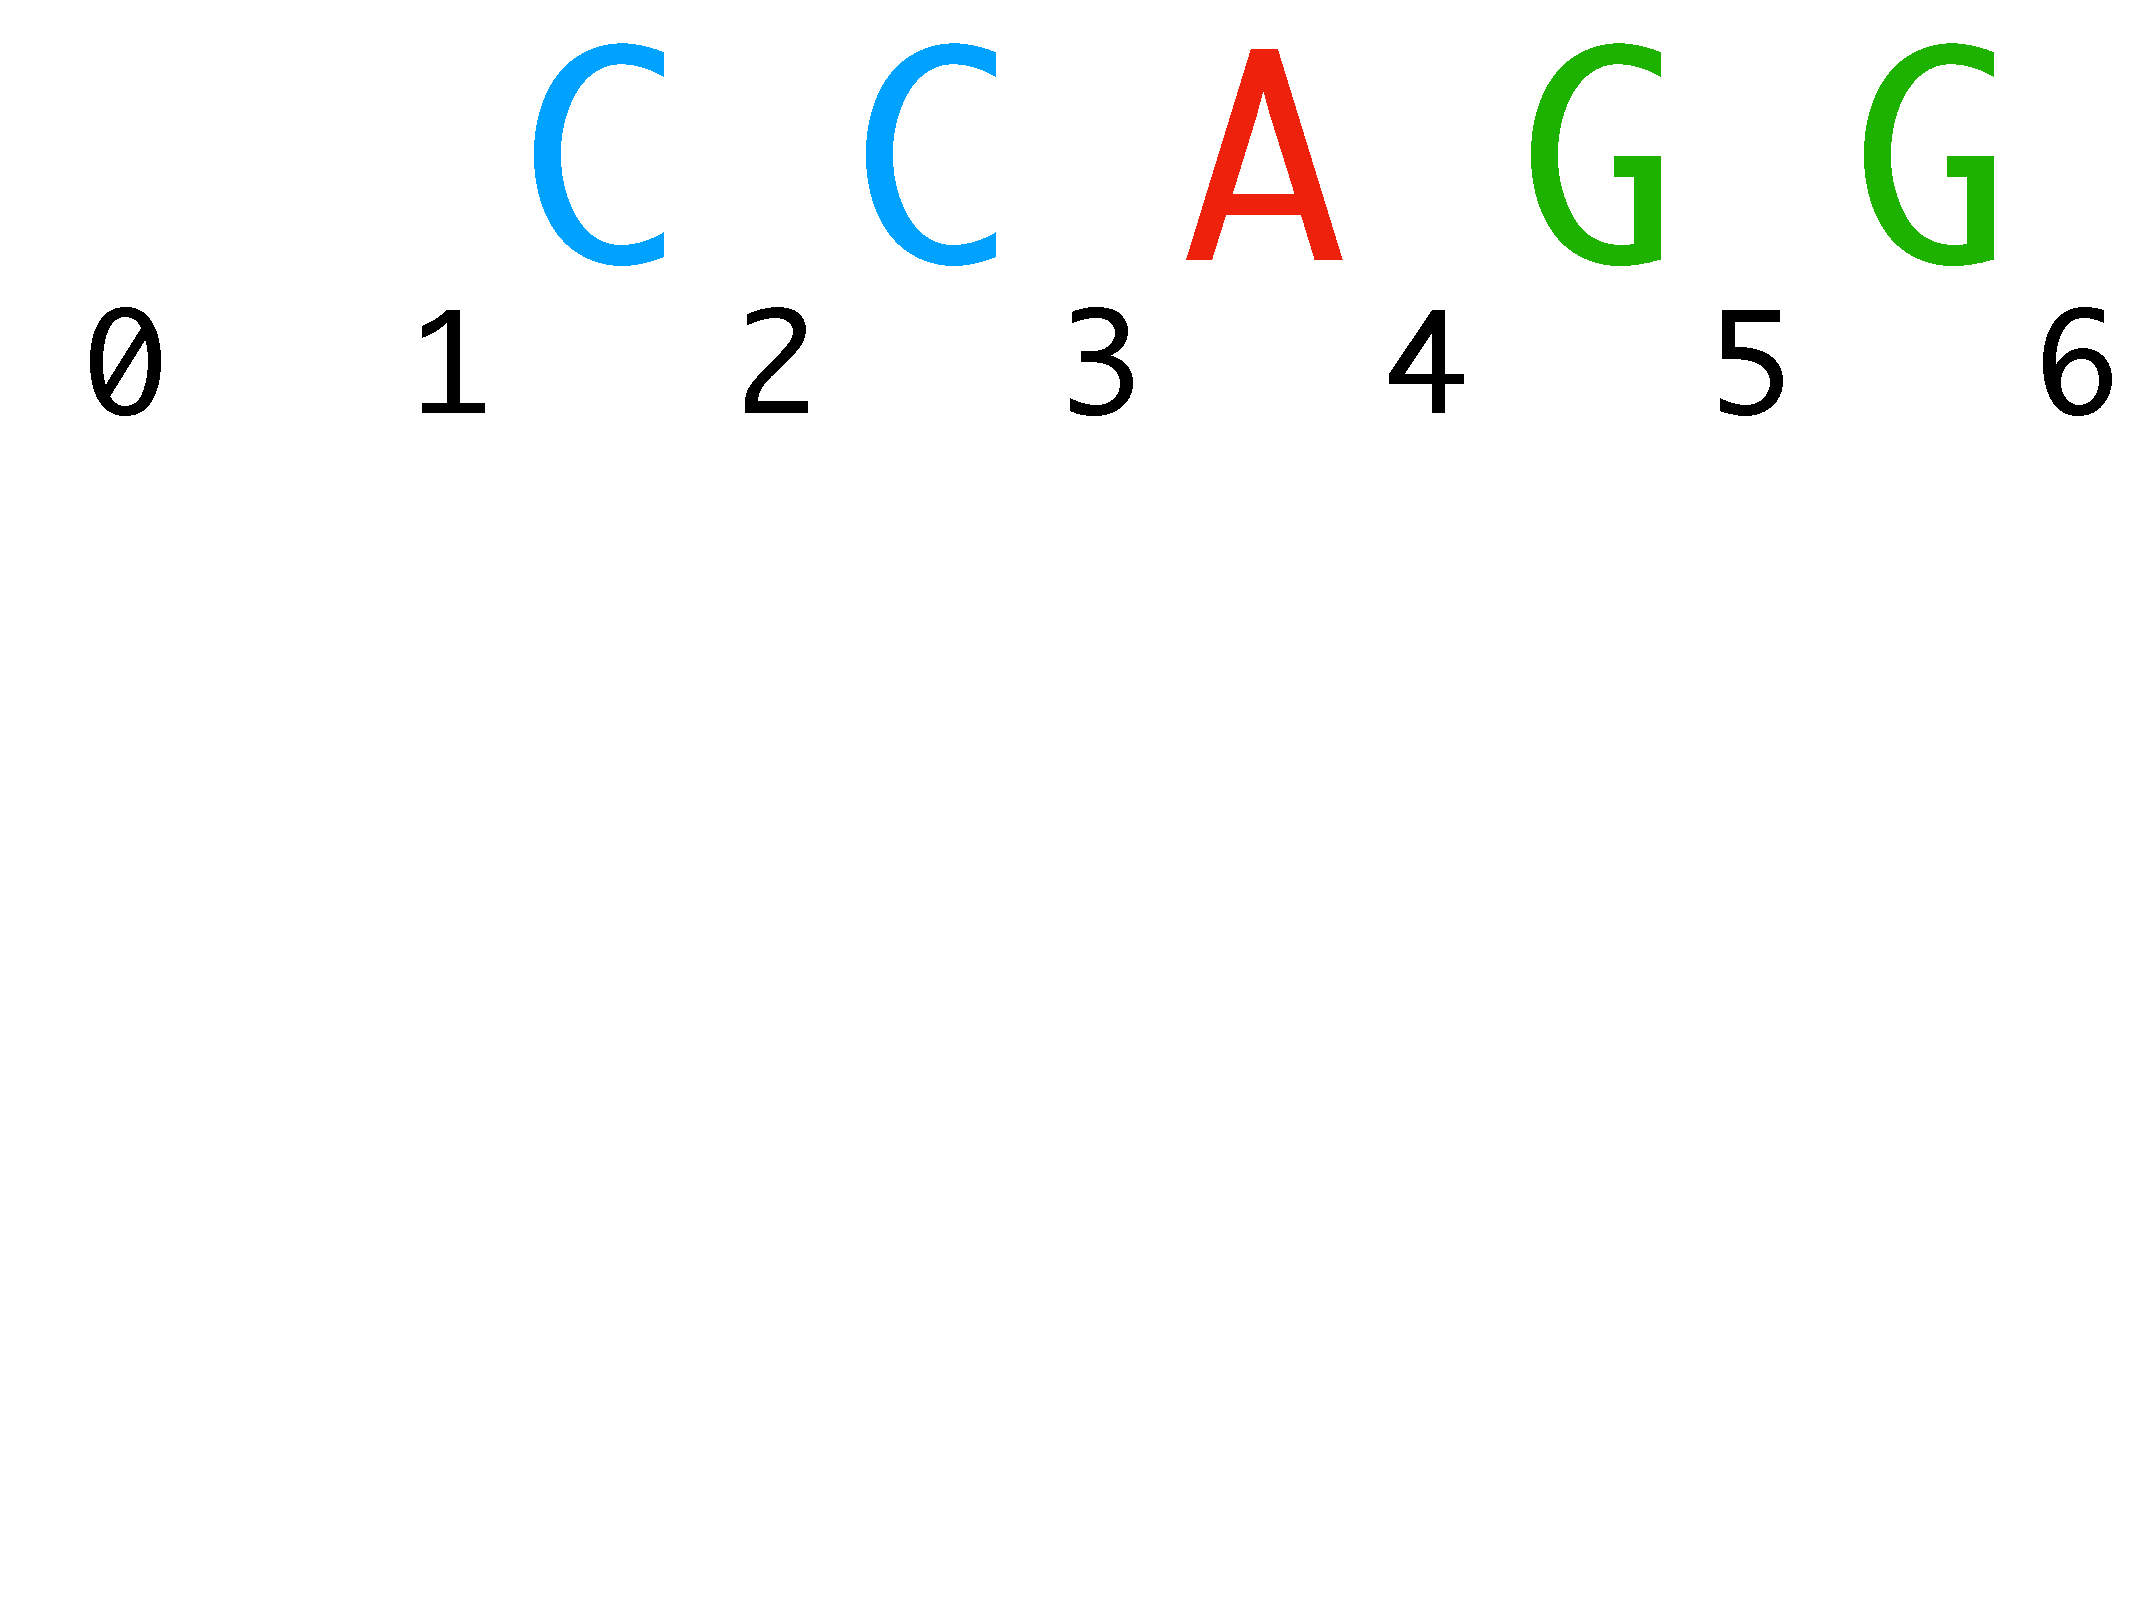
\includegraphics[scale=.16]{figs/index} \\[-3.cm]
%\hspace{-0.23cm}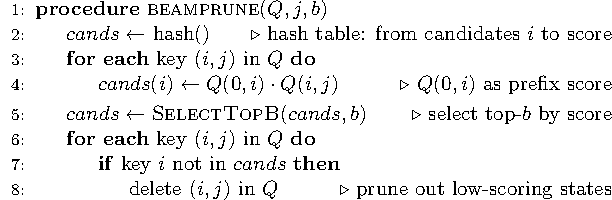
\includegraphics[scale=1.2]{figs/beam_prune_alg} \\[0.5cm]
  \algrenewcommand\algorithmicindent{1.5em}%
\begin{minipage}{0.85\textwidth}
\begin{algorithmic}[1]
  \newcommand{\INDSTATE}[1][1]{\State\hspace{#1\algorithmicindent}}
  \setstretch{1.2} % lhuang: usepackage setspace
\Function{beamprune}{$Q, j, b$}
    \State $\candidates \gets$ hash() \Comment{hash table: from candidates $i$ to score}
    \ForEach{$i$ such that $[i,j]$ in $Q$}
        \State $\candidates[i] \gets \Qf{1}{i-1} \cdot \Qf{i}{j}$ \Comment{like \linearfold, use $\Qf{1}{i-1} $ as prefix score}
    \EndFor
    \State $\candidates \gets \textsc {SelectTopB}(candidates, b)$ \Comment{select top-$b$ states by score}
    \ForEach{$i$ such that $[i,j]$ in $Q$}
        \If{key $i$ not in $candidates$}
            \State {\bf delete} $[i,j]$ from $Q$ \Comment{prune low-scoring states}
        \EndIf
    \EndFor
\EndFunction
\end{algorithmic}
% \end{algorithm}
\end{minipage}
\caption{
The {\sc BeamPrune} function from the Pseudocode of our main algorithm (Fig.~\ref{fig:algorithm}).
\label{fig:beam_prune_alg}}
% \vspace{-0.3cm}
% \end{figure*}
\end{figure}x


\begin{figure}[h]%[b]
  % \newcommand{\pluseq}{\mathrel{+}=}
\center
\small
\algrenewcommand\algorithmicindent{1.5em}%
  % \algnewcommand\algorithmicforeach{\textbf{for each}}
\algdef{S}[FOR]{ForEach}[1]{\algorithmicforeach\ #1\ \algorithmicdo}
% \hspace{-0.23cm}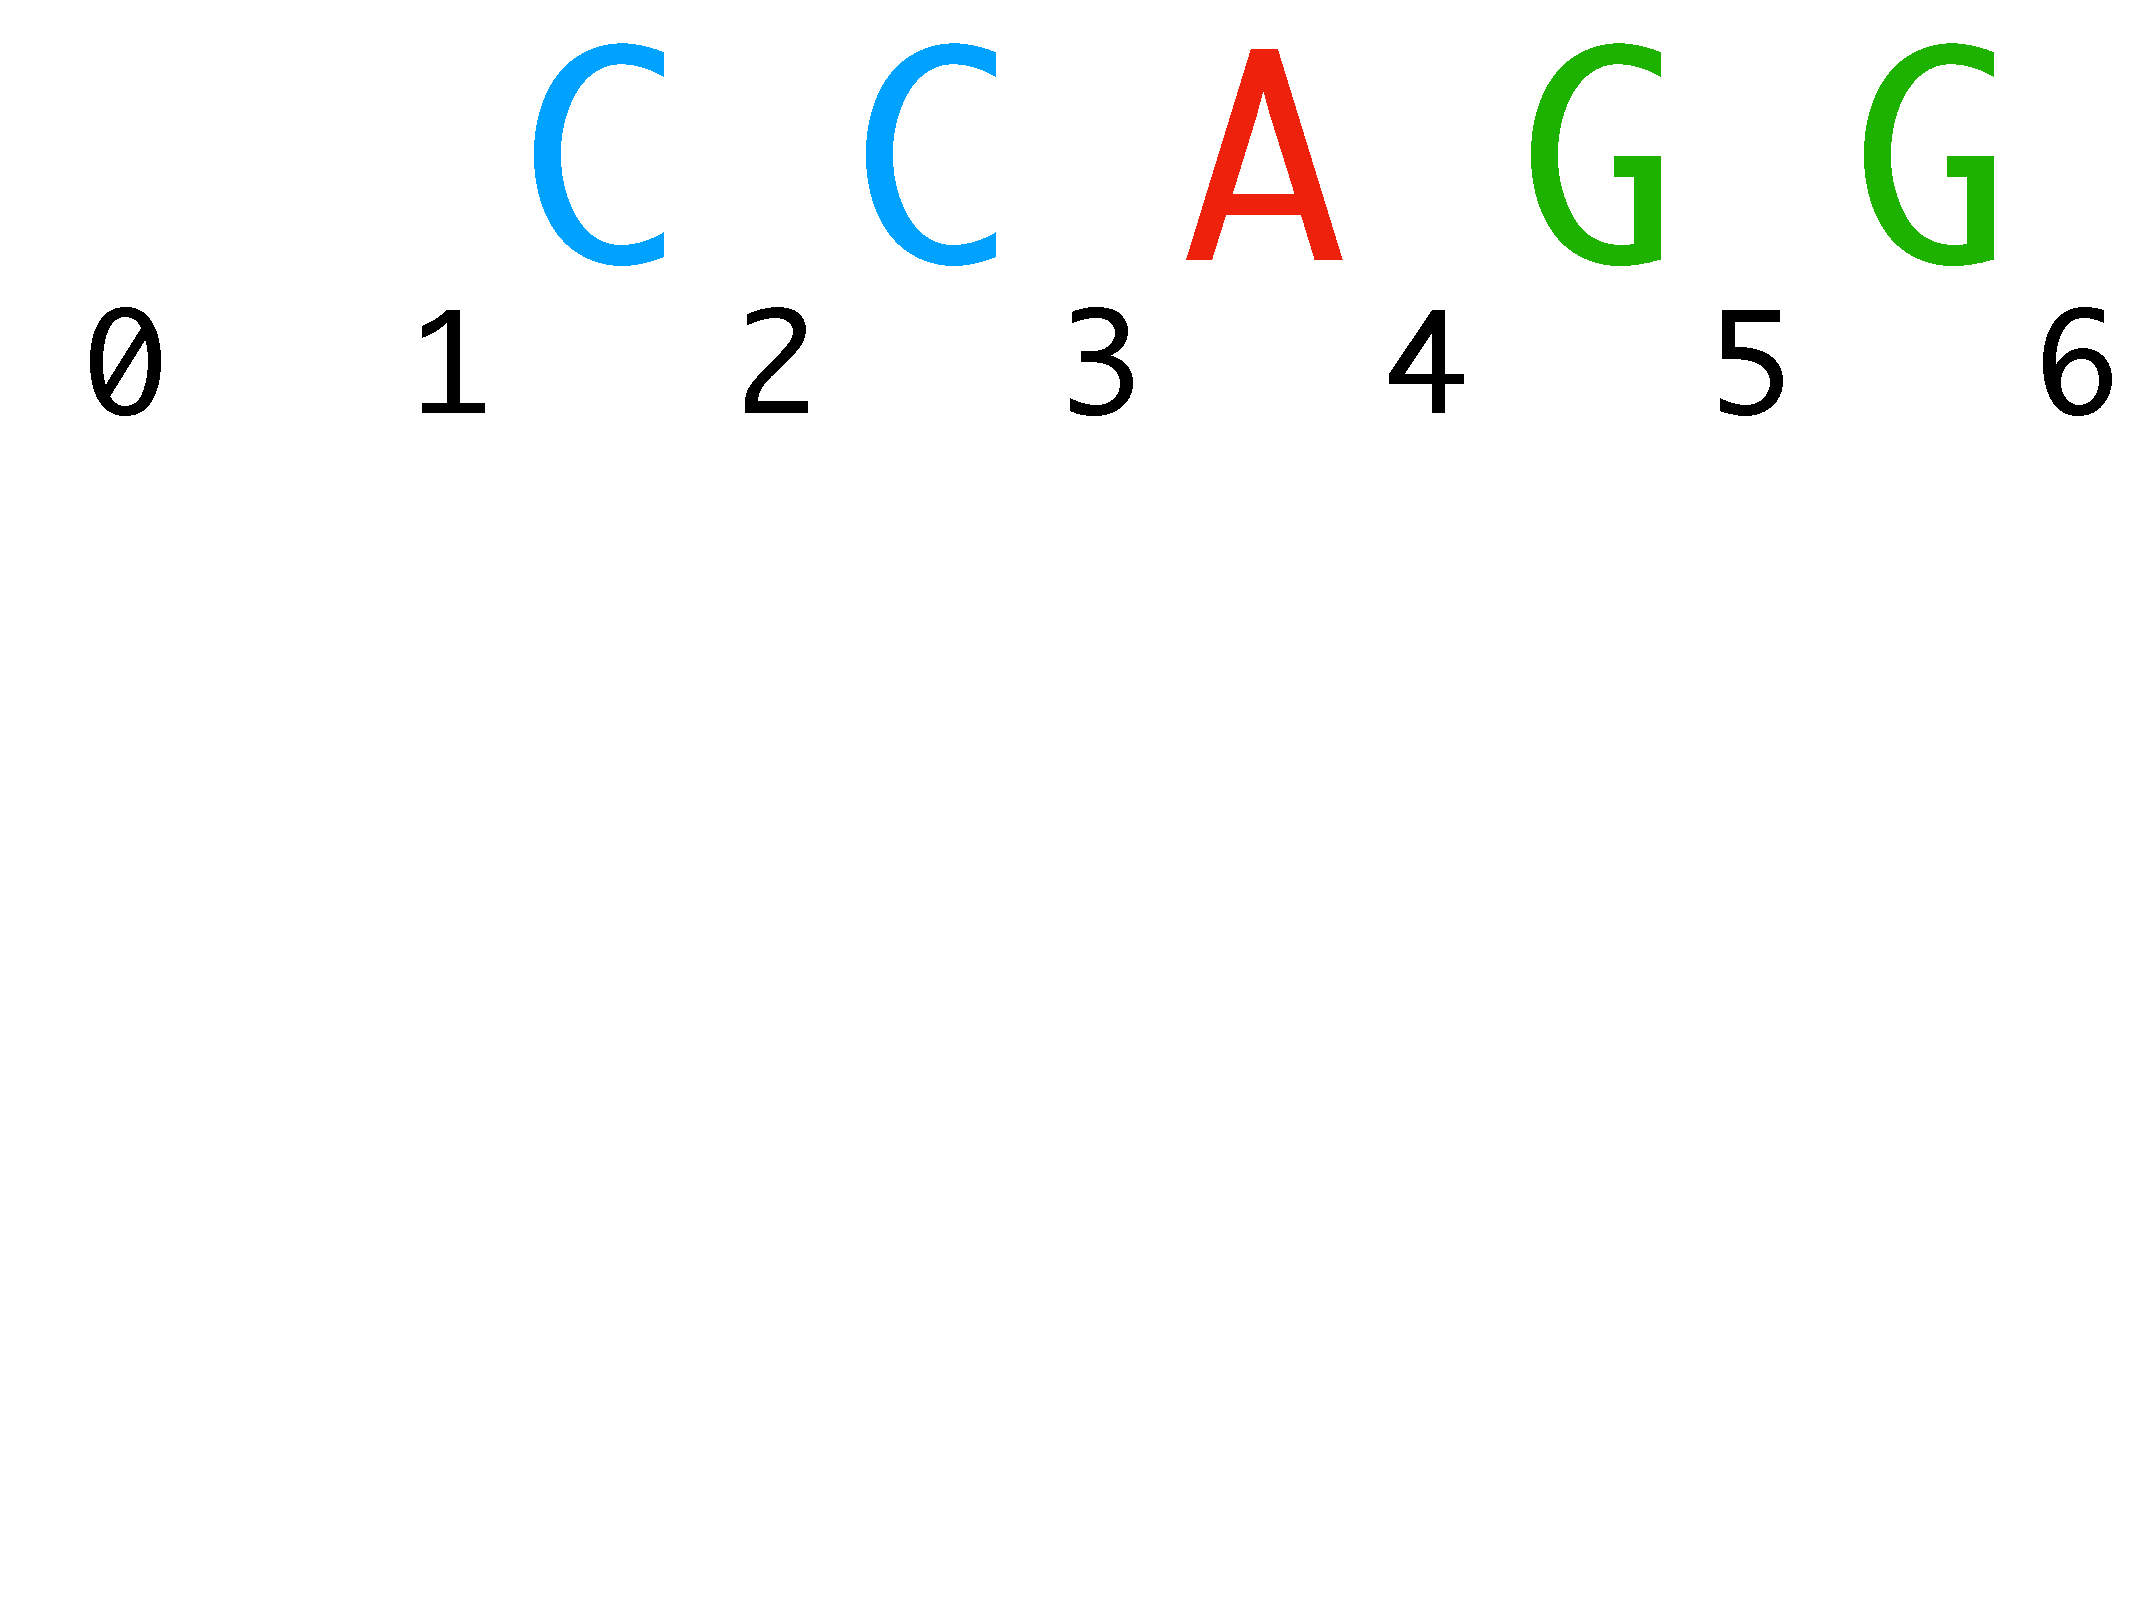
\includegraphics[scale=.16]{figs/index} \\[-3.cm]
%\hspace{-0.23cm}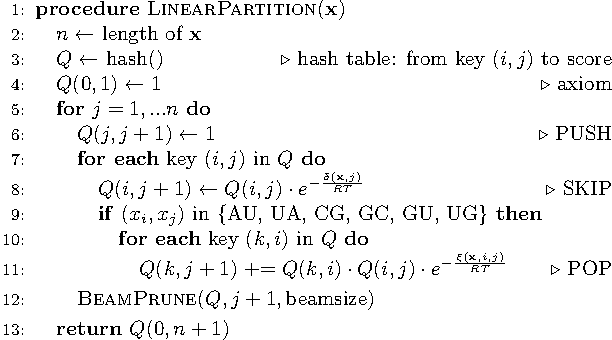
\includegraphics[scale=.83]{figs/algorithm} \\[0.2cm]
\begin{minipage}{.85\textwidth}
\begin{algorithmic}[1]
  \newcommand{\INDSTATE}[1][1]{\State\hspace{#1\algorithmicindent}}
  \setstretch{1.2} % lhuang: usepackage setspace
\Function{BasePairingProbs}{$\vecx, Q$}  \Comment{outside calculation}
% \bindent
    \State $n \gets$ length of $\mathbf x$
    \State $\Qhat \gets$ hash() \Comment{hash table: from span $[i,j]$ to $\Qhatf{i}{j}$: outside partition function}
    \State $p \gets$ hash() \Comment{hash table: from span $[i,j]$ to $p_{i,j}$: base-pairing probs}
    % \State $Q[j,\,j-1] \gets 1$ for all $j$ in $1...n$ \Comment{base cases} \label{line:base}
    \State $\Qhatf{1}{n} \gets 1$ \Comment{base case}
    \For{$j=n$ {\bf downto } $1$}
        \ForEach {$i$ such that $[i,\,j-1]$ in $Q$}\smallskip
            \State $\Qhatf{i}{j-1} \pluseq \Qhatf{i}{j} \cdot e^{-\frac{\delta(\vecx,j)}{RT}} $ \Comment{\nskip} \label{line:skip}
            \If{$x_{i-1}x_j$ in \{AU, UA, CG, GC, GU, UG\}}  \label{line:pair}
                % \State $Q_{i,\,j+1} \gets  C(i,\,j) \cdot e^{-\frac{\xi(\vecx,i,\,j)}{RT}} $
                \ForEach{$k$ such that $[k,\,i-2]$ in $Q$}\smallskip
                    \State $\Qhatf{k}{i-2} \pluseq {\Qhatf{k}{j} \cdot \Qf{i}{j-1} \cdot e^{-\frac{\xi(\vecx,i-1,j)}{RT}}}$ \Comment{\pop: left} %\label{line:pop}
                    % \State $C(0,j+1) \pluseq {C(0,k) \cdot C(k,j+1) \cdot e^{-\frac{\xi(\vecx,i,\,j)}{RT}}} $
                    \State $\Qhatf{i}{j-1} \pluseq {\Qhatf{k}{j} \cdot \Qf{k}{i-2} \cdot e^{-\frac{\xi(\vecx,i-1,j)}{RT}}}$ \Comment{\pop: right} %\label{line:pop}
                    \State $p_{i-1,\,j} \pluseq \displaystyle\frac{\Qhatf{k}{j} \cdot \Qf{k}{i-2}  \cdot  e^{-\frac{\xi(\vecx,i-1,j)}{RT}} \cdot \Qf{i}{j-1}}{\Qf{1}{n}}$ \Comment{accumulate base pairing probs}
                \EndFor
                % \State $C(0,j+1) \pluseq C(0,i) \cdot Q_{i,j+1}$ \Comment{COMBINE}
            \EndIf
        \EndFor
        %% \ForEach {$i$ such that $[i,\,j]$ in $P$}\smallskip
        %%          \State $p_{i,j} = \frac{\hatp[i,\,j] \cdot Q[i+1,\, j-1]}{Q[1,n]}$
        %% \EndFor
        % \State $\textsc {BeamPrune}(Q,j+1, b)$ \Comment{see Fig.~\ref{fig:beam_prune_alg}}
    \EndFor
    \State \Return $p$ \Comment{return the (sparse) base-pairing probability matrix}
% \eindent
\EndFunction
%% \Function{BasePairingProbabilities}{$\vecx, Q, \hatp$} % \Comment{$Q$ is the beam size}
%% % \bindent
%%     \State $p \gets$ hash() \Comment{hash table: from span $[i,j]$ to base pairing probability $p_{i,j}$}
%%     \For{$j=2 ... |\vecx|$}
%%       \ForEach {$i$ such that $[i,j]$ in $\hatp$}
%%           \State $p_{i,j} = \displaystyle\frac{\hatp[i,\,j] \cdot Q[i+ 1,\, j-1] \cdot  e^{-\frac{\xi(\vecx,i,j)}{RT}}}{Q[1,n]}$
%%       \EndFor
%%     \EndFor
%%     \State \Return the (sparse) base-pairing probability matrix $p$
%% \EndFunction
\end{algorithmic}
\end{minipage}
\caption{
  Outside partition function and base pairing probabilities calculation for a simplified version of the \linearpartition.
  $Q$ is the (inside) partition function calculated by the pseudocode in Fig.~\ref{fig:algorithm}, and $\Qhat$ is the outside partition function. 
% as well as a beam prune algorithm. 
% Here we model hash tables following Python dictionaries, where $(i, j) \in C$ checks whether the key $(i, j)$ is in the hash $C$; 
% this is needed to ensure linear runtime. 
% Quick select algotithm is used in beam prune, 
% and we skip the details for quick select here since it is well known.
% Real \linearpartition system is much more involved, but the pseudocode illustrates the left-to-right partition function calculation idea using a Nussinov-like fashion.
The actual algorithm using the Turner model is in our \href{https://github.com/LinearFold/LinearPartition}{GitHub codebase}.
%See Fig.~\ref{fig:beam_prune_alg} for {\sc BEAMPRUNE} function.
\label{fig:outside}}
\vspace{-0.3cm}
% \end{figure*}
\end{figure}


\iftrue
\begin{figure}[h]
  \centering
  \captionsetup{singlelinecheck=off}
%\hspace{-0.5cm}
\begin{tabular}{ll}
\hspace{-.5cm}{\panel A} & {\panel B}\\[-1cm]
    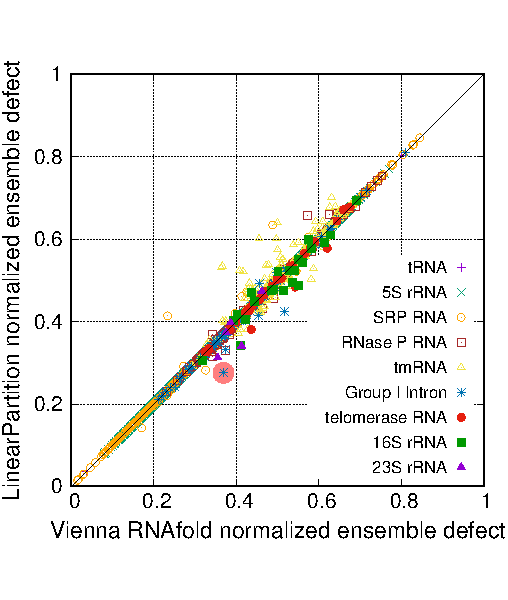
\includegraphics[width=.3\textwidth]{figs/norm_ensemble_defect}
    &
    \hspace{-0.1cm}
    \raisebox{.5cm}{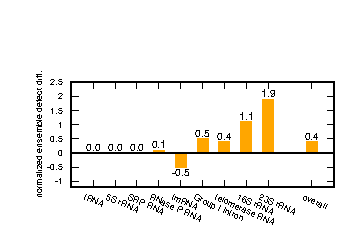
\includegraphics[width=.5\textwidth]{figs/onebar_norm_ensemble_defect_histogram}}
  \end{tabular} \\[-.3cm]
  \caption[.]{
  The 
  comparison of normalized ensemble defects (normalized by sequence length)
  % between \viennarnafold and \linearpartitionv 
  on the ArchiveII dataset.
  % Ensemble defects are normalized by sequence length. 
  {\bf A}: 
  Normalized ensemble defect between \viennarnafold and \linearpartitionv for each sequence; the trend is similar as Fig.~\ref{fig:ensemble}A, but the deviations for tmRNAs are more apparent; 
  the point with red shaded are the example in Fig.~\ref{fig:example}.
  {\bf B}: Normalized ensemble defect difference for each family; for longer families, 
  e.g., Group I Intron, telomerase RNA, 16S and 23S rRNA, 
  \linearpartition has lower normalized ensemble defect differences;
  note that \linearpartition's normalized ensemble defects are significantly better than \viennarnafold on Group I Intron ($p < 0.01$), 
  but significantly worse on tmRNA ($p < 0.01$).
  \label{fig:ensemble_defect}}
%\vspace{1cm}
\end{figure}
\fi

\iffalse
\begin{figure}[h]
  \centering
  \captionsetup{singlelinecheck=off}
\begin{tabular}{cccc}
\hspace{-4.4cm} \panel{A} & \hspace{-4.6cm}\panel{B} & \hspace{-4.6cm}\panel{C} & \hspace{-4.6cm}\panel{D}\\[-0.2cm]
\hspace{-0.2cm}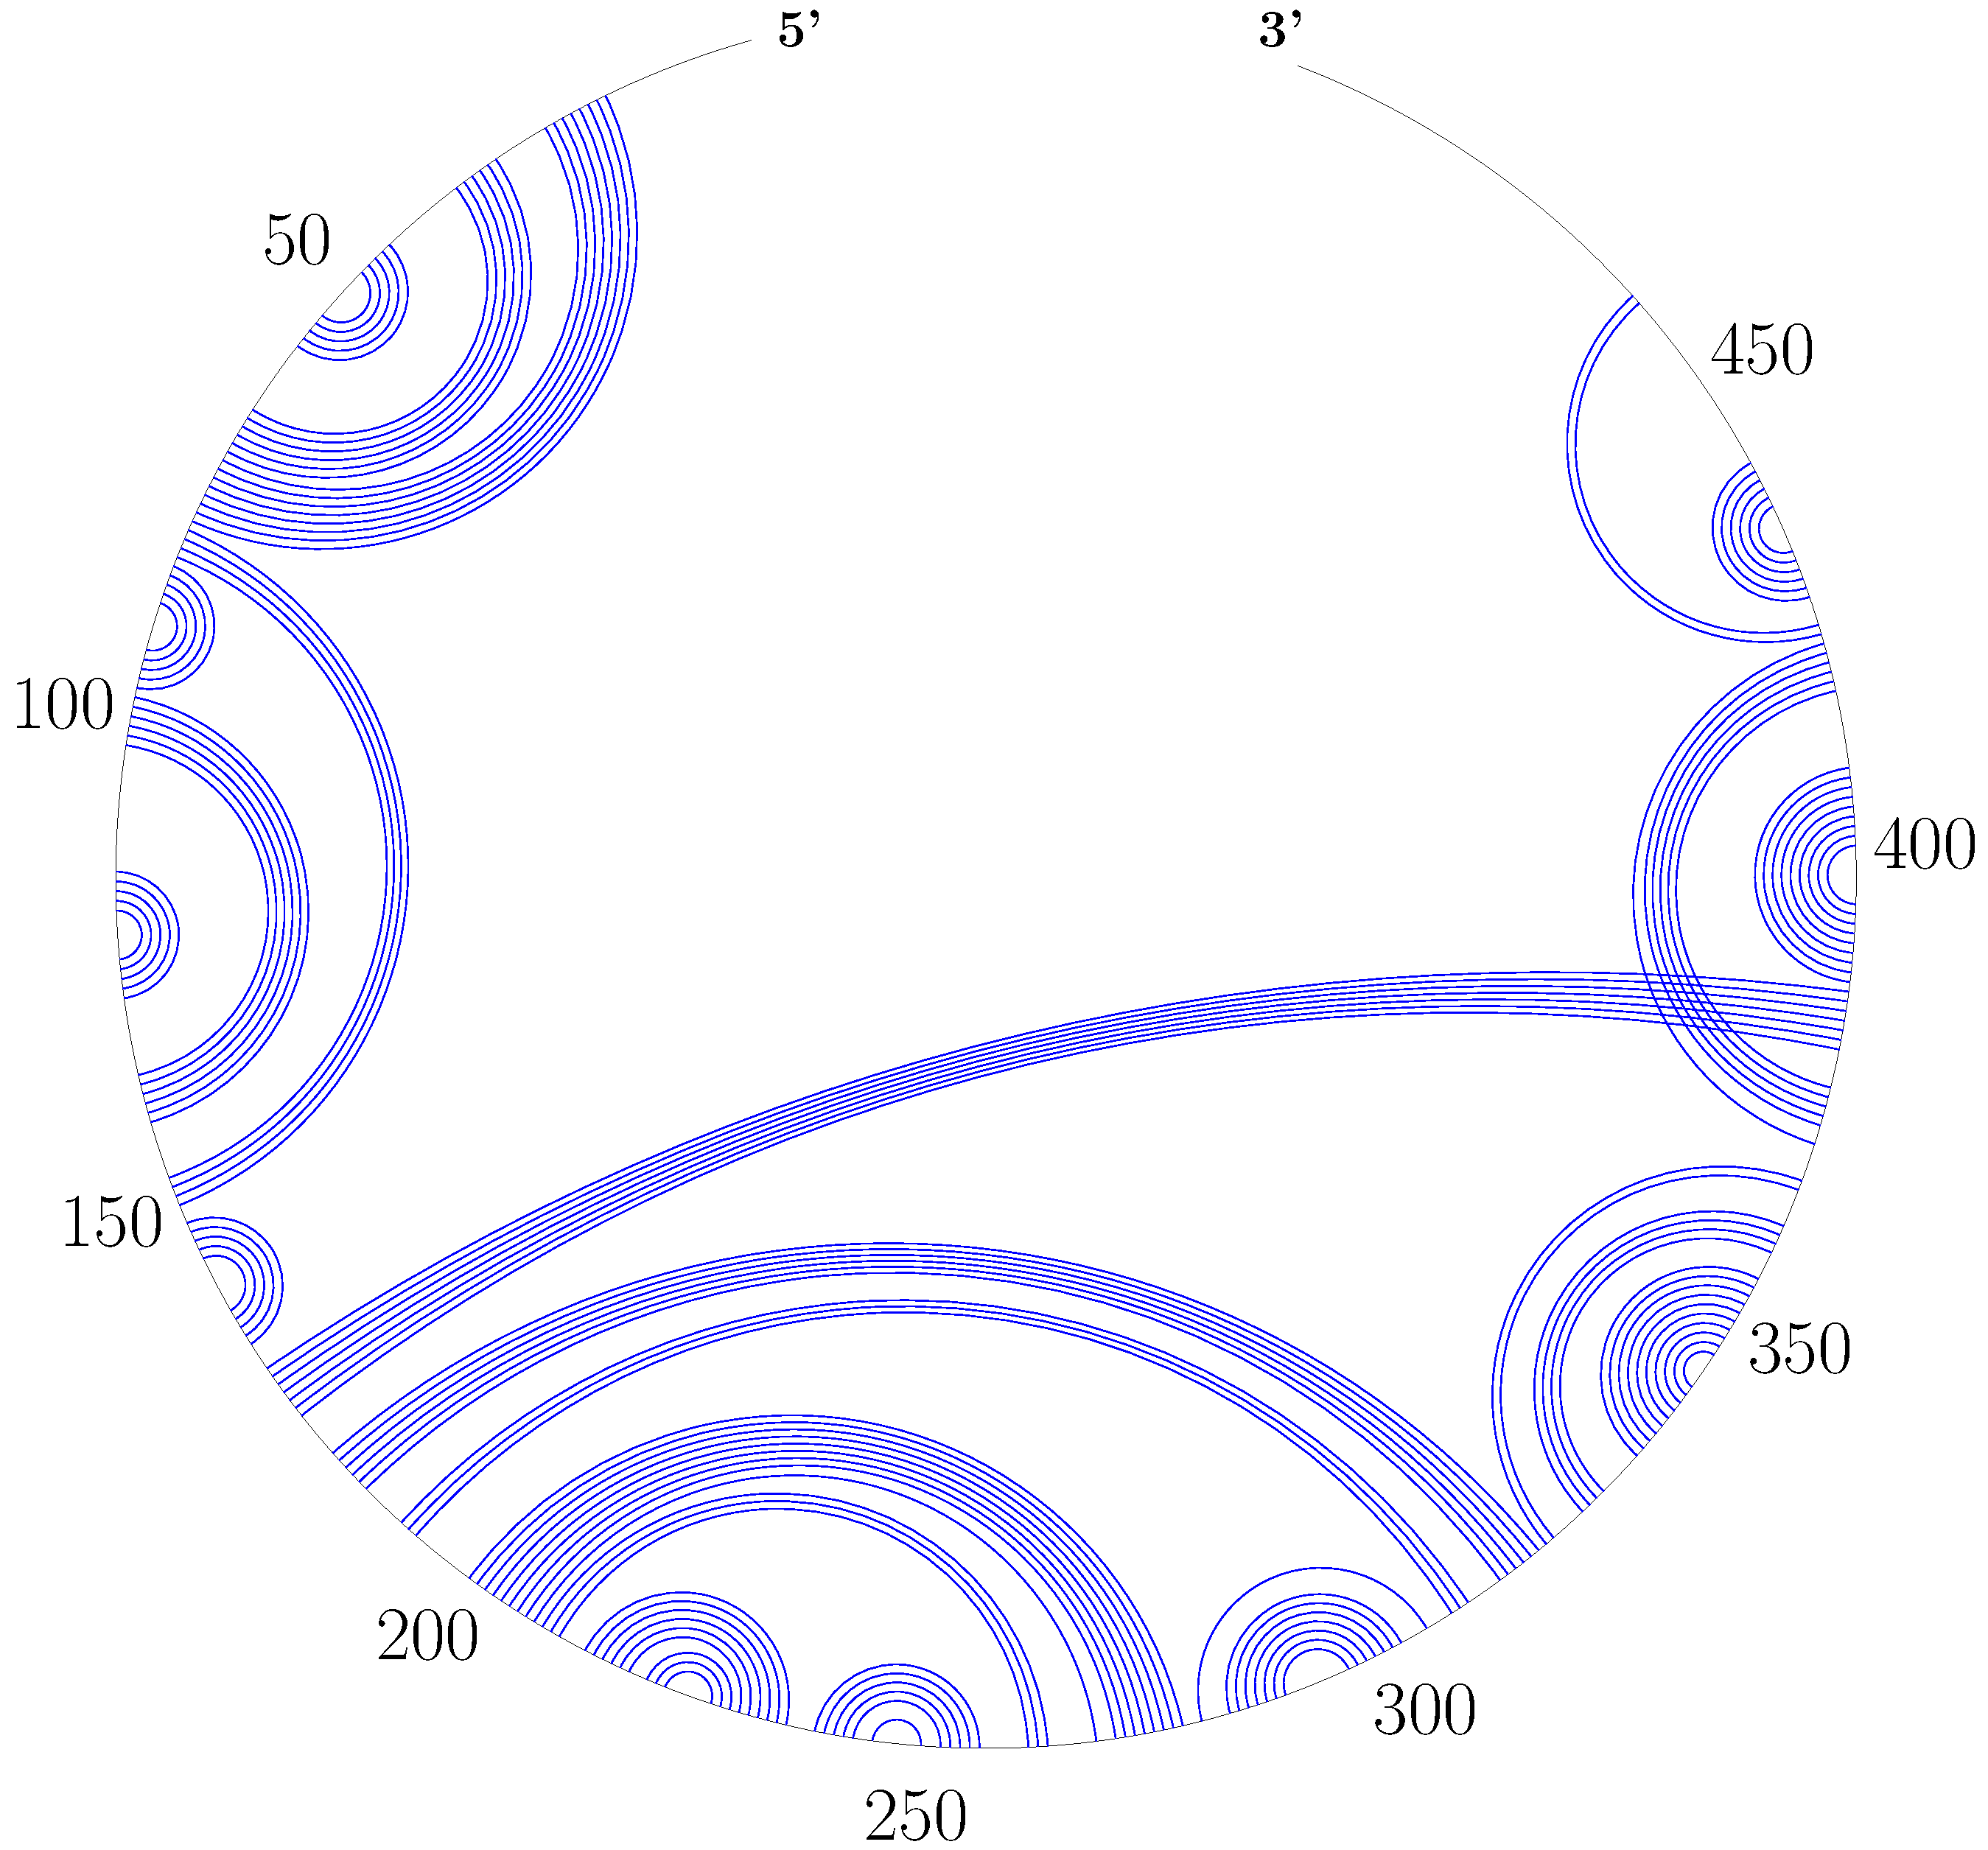
\includegraphics[width=0.25\textwidth]{figs/grp1_gold} &
\hspace{-0.35cm}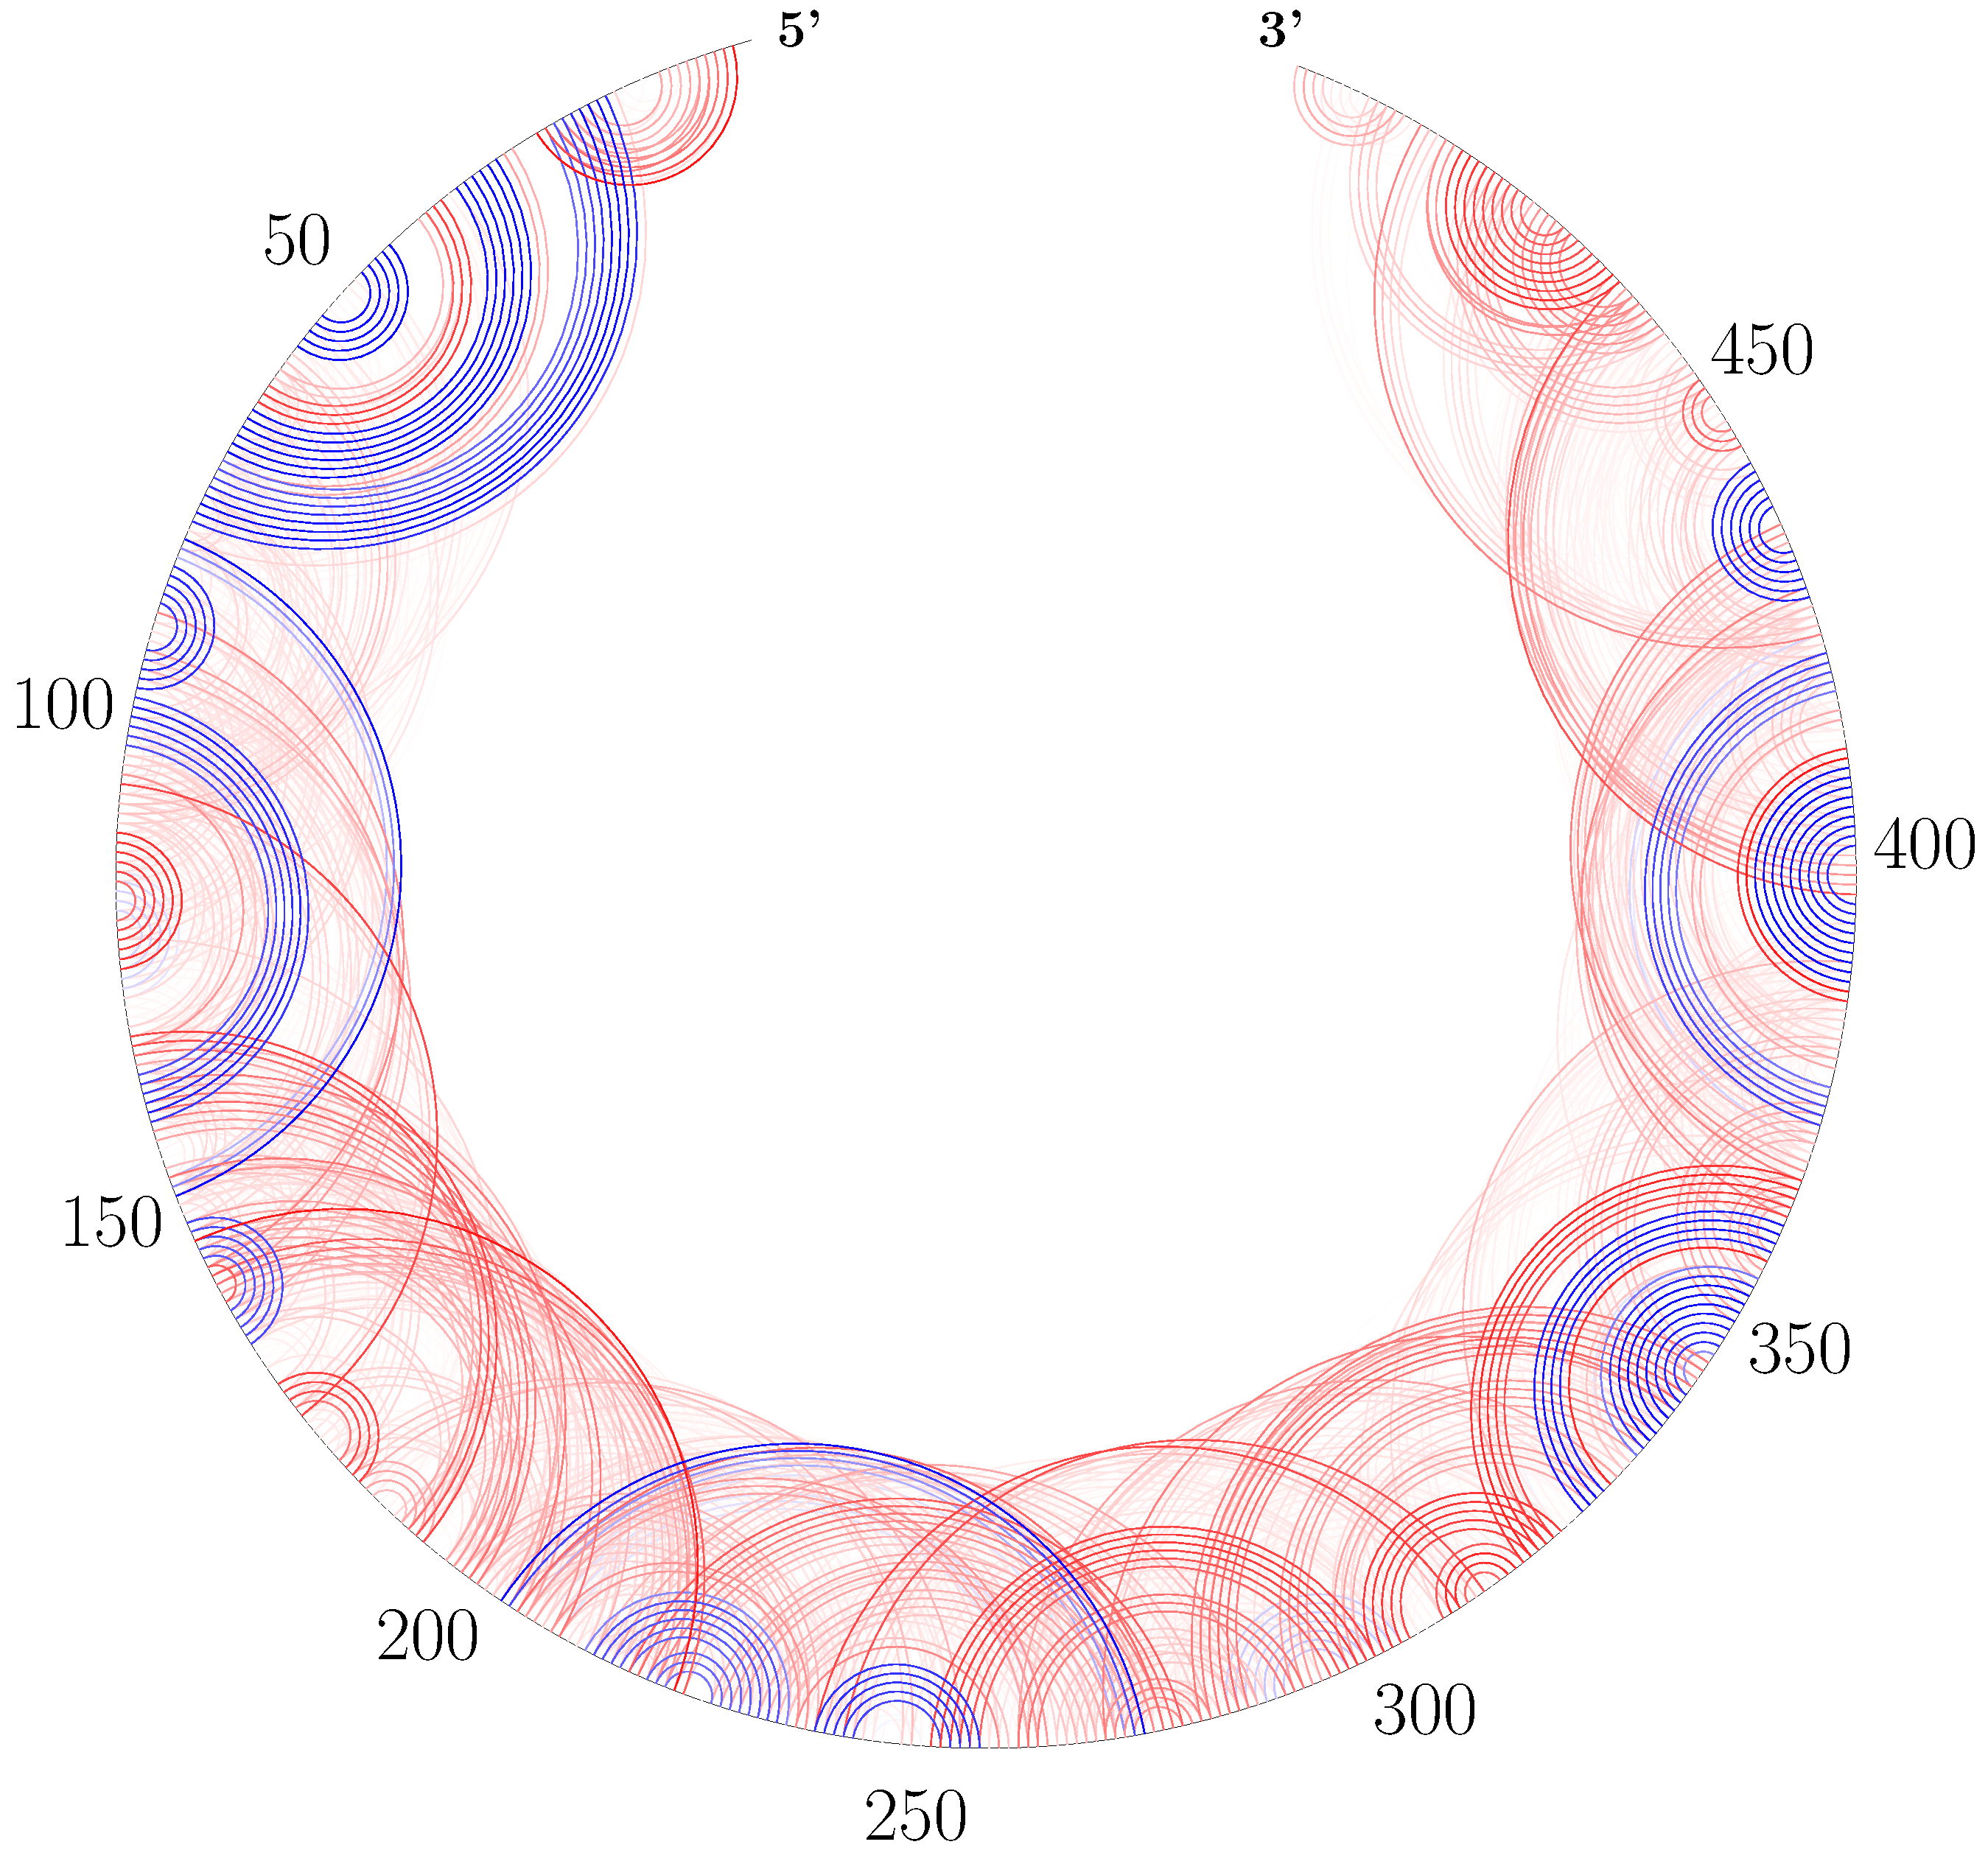
\includegraphics[width=0.25\textwidth]{figs/grp1_vienna_plfold_example.pdf} &
\hspace{-0.35cm}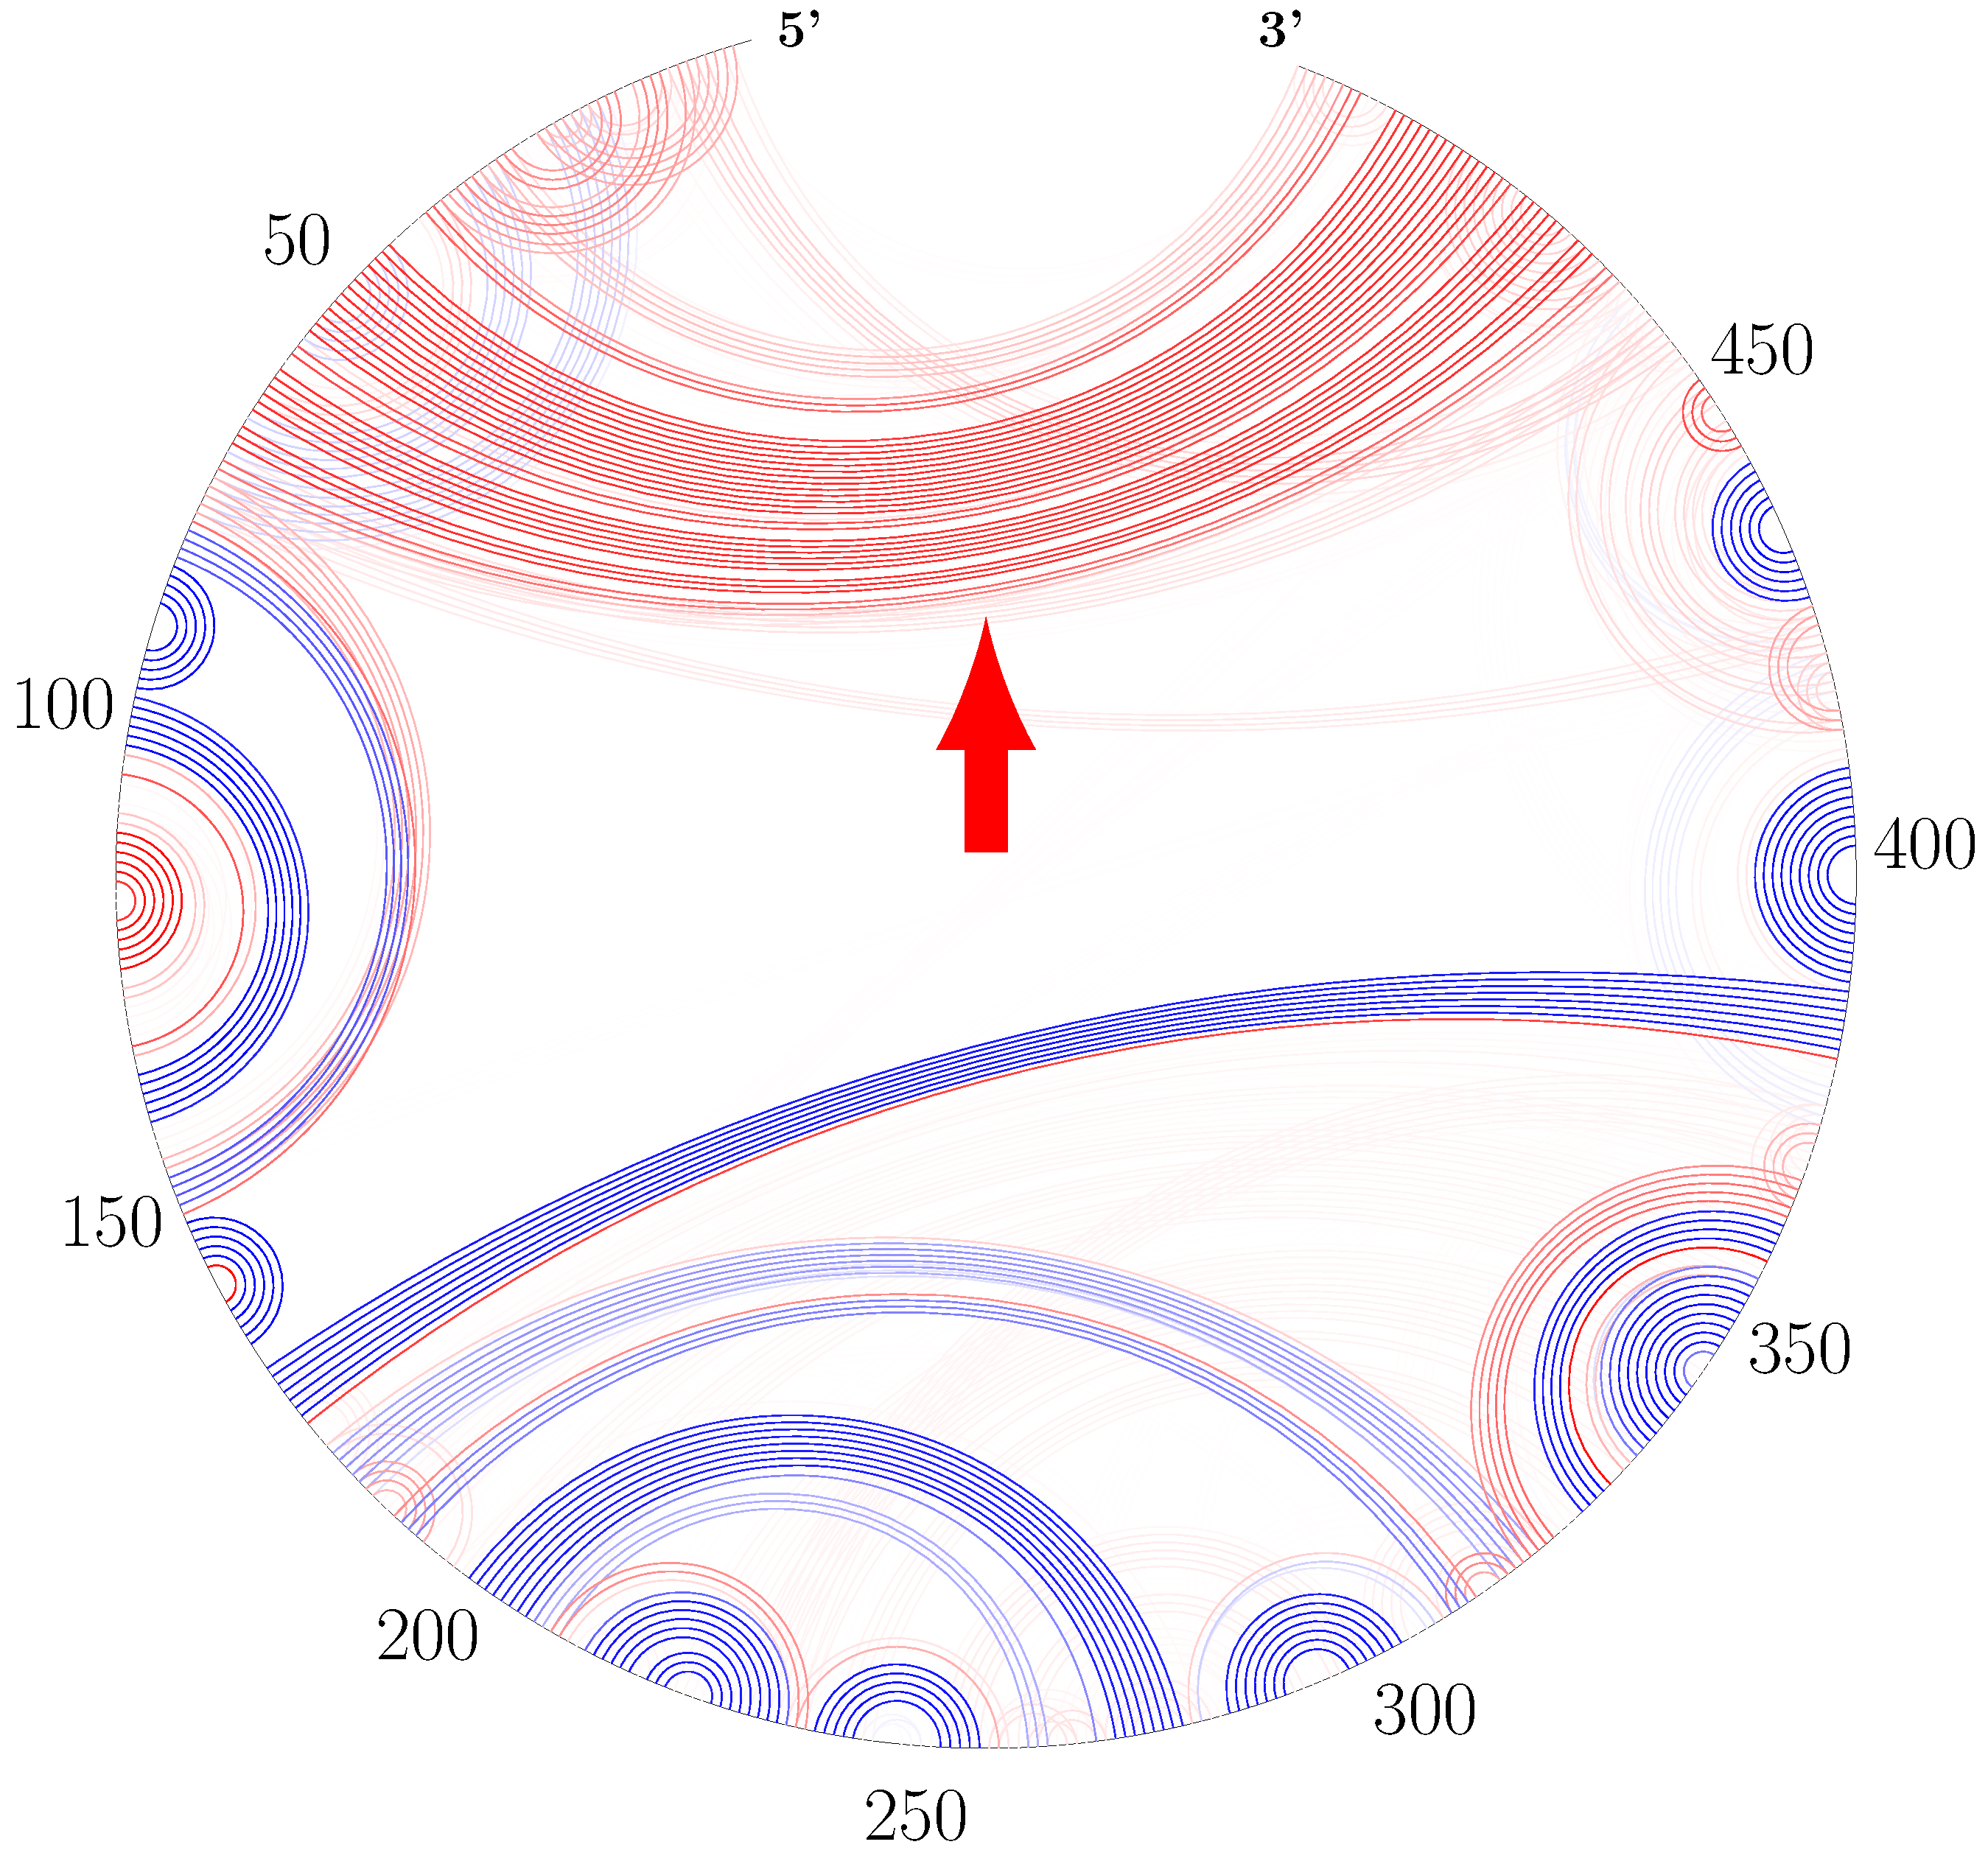
\includegraphics[width=0.25\textwidth]{figs/grp1_vienna_example} &
\hspace{-0.35cm}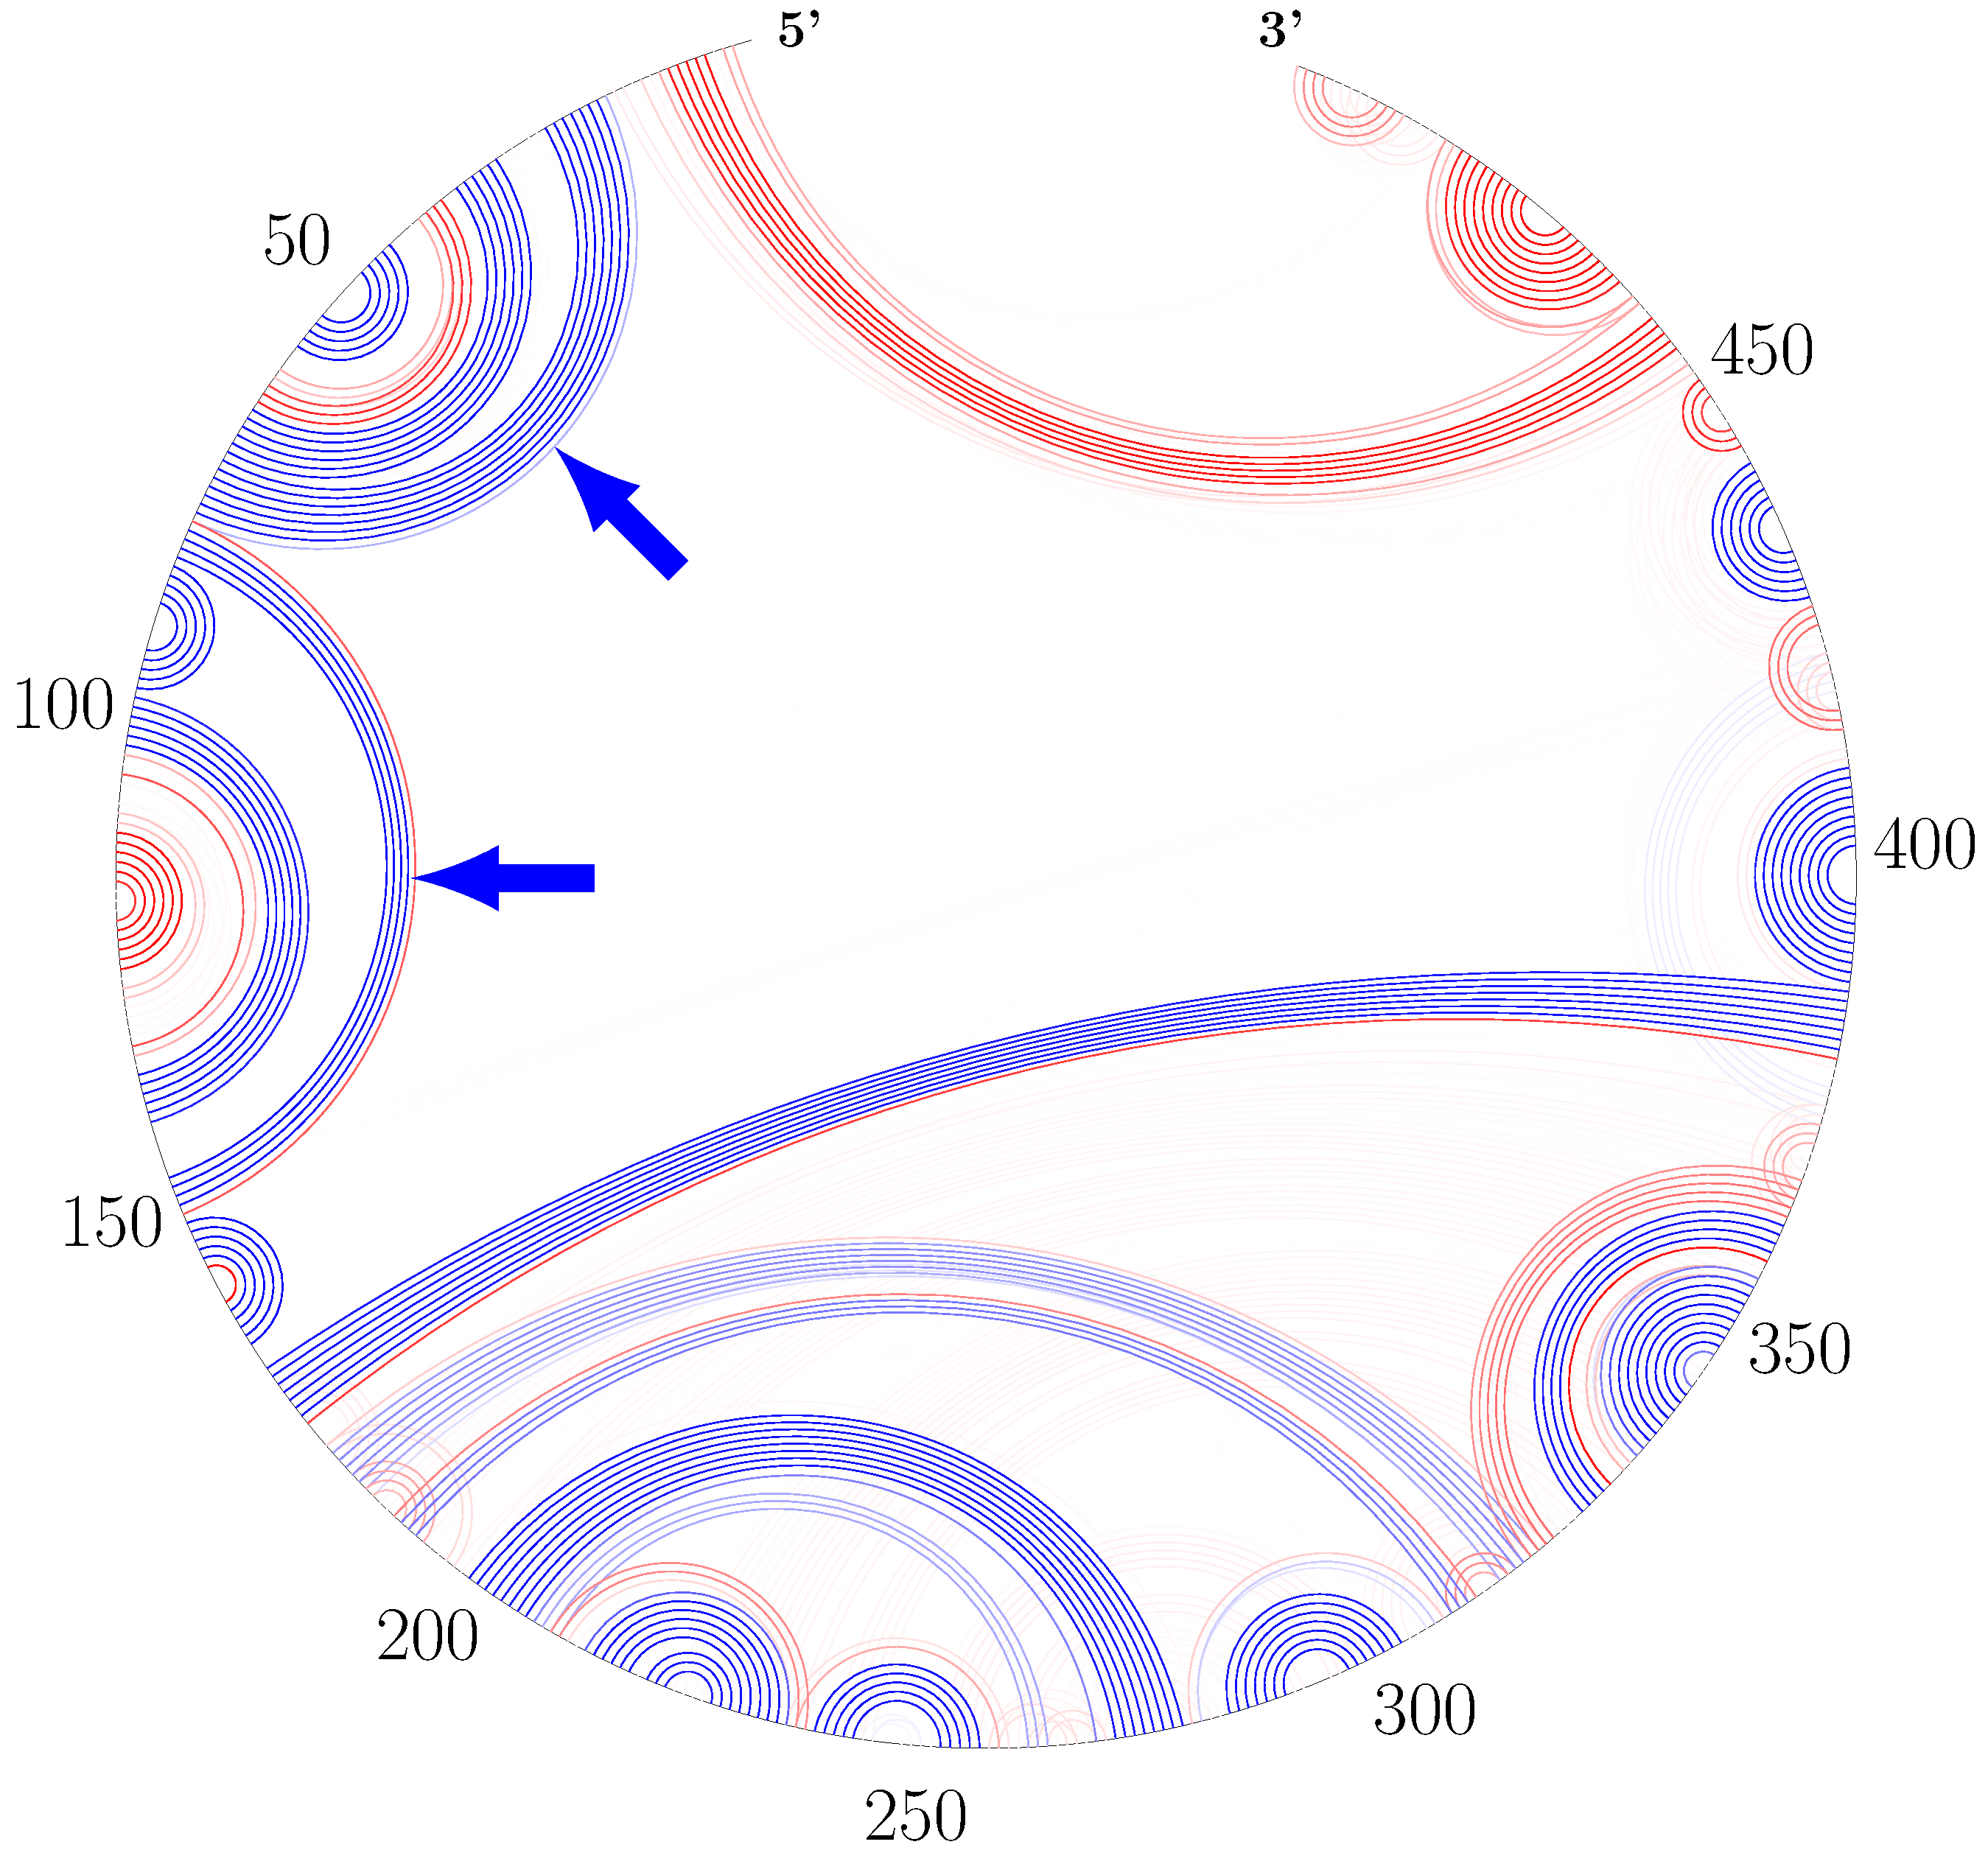
\includegraphics[width=0.25\textwidth]{figs/grp1_lpv_example.pdf}
\end{tabular}
  \caption[.]{Circular plots of {\it C.~ellipsoidea} Group I Intron.  
  Blue denotes pairs in the known structure and Red denotes predicted pairs not in the known structure.  
  The darkness of the line indicates pairing probability, 
  which the darkest lines close to a portability of 1. 
  {\bf A}: 
  [Please explain what is shown in each panel.] [I also think a key with blue and red in the figure would be helpful here as well.]
  \label{fig:circular_grp1}}
%\vspace{1cm}
\end{figure}
\fi

%\newpage
% mea
\iftrue
\begin{figure}[h]
  \centering
%\hspace{-0.5cm}
\begin{tabular}{ll}
{\large\sf A} & {\large\sf B}\\[-1cm]
    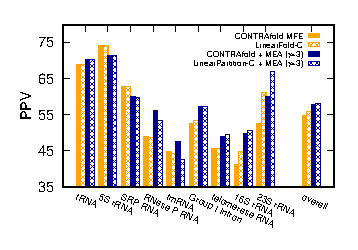
\includegraphics[width=.45\textwidth]{figs/MEA_vs_MFE_PPV_LPC}
    &
    \hspace{-0.1cm}
    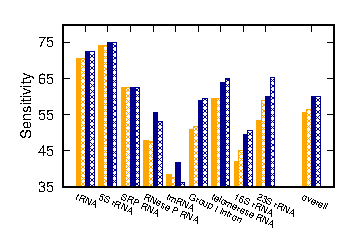
\includegraphics[width=.45\textwidth]{figs/MEA_vs_MFE_sens_LPC}
  \end{tabular} \\[-0.5cm]
  \caption{Accuracy comparison of MEA structures ($\gamma=3$) between \contrafold and \linearpartitionc on the ArchiveII dataset. 
  $\gamma$ is the hyperparameter balances PPV and Sensitivity. Note that \linearpartitionc + MEA is significantly worse than \contrafold + MEA on two families in both PPV and Sensitivity, tmRNA and RNase P RNA ($p < 0.01$).
  \label{fig:mea_lpc}}
%\vspace{1cm}
\end{figure}
\fi

% threshknot
\iftrue
\begin{figure}[h]
  \centering
%\hspace{-0.5cm}
\begin{tabular}{ll}
{\large\sf A} & {\large\sf B}\\[-1cm]
    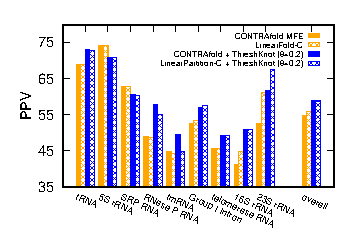
\includegraphics[width=.45\textwidth]{figs/new_ThreshKnot_vs_MFE_PPV_LPC}
    &
    \hspace{-0.1cm}
    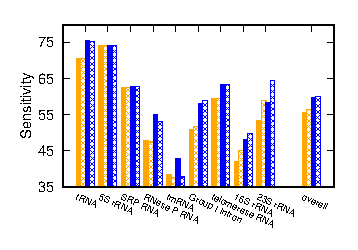
\includegraphics[width=.45\textwidth]{figs/new_ThreshKnot_vs_MFE_sens_LPC}
  \end{tabular} \\[-0.5cm]
  \caption{Accuracy comparison of ThreshKnot structure ($\theta=0.2$) between \contrafold and \linearpartitionc on ArchiveII dataset. $\theta$ is the hyperparameter that balances PPV and Sensitivity. Note that \linearpartitionc + ThreshKnot is significantly worse than \contrafold + ThreshKnot on two families in both PPV and Sensitivity, tmRNA and RNase P RNA ($p < 0.01$), and significantly better on three longer families in Sensitivity, Group I Intron ($p < 0.01$), telomerase RNA and 16S rRNA ($0.01 \leq p < 0.05$).
  \label{fig:threshknot_lpc}}
%\vspace{1cm}
\end{figure}
\fi


\begin{figure}[h]
  \centering
  \captionsetup{singlelinecheck=off}
\begin{tabular}{cc}
\hspace{-6.cm} \panel{A} & \hspace{-6cm}\panel{B} \\[-0.5cm]%& \hspace{-4.6cm}\panel{C} & \hspace{-4.6cm}\panel{D}\\[-0.2cm]
\hspace{-0.2cm}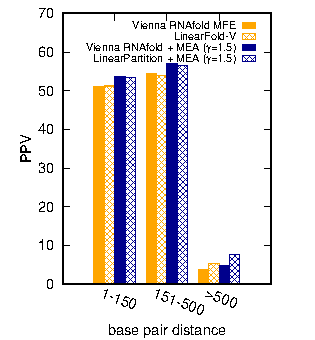
\includegraphics[width=0.35\textwidth]{figs/bylen_bar_precision_hzhang} &
\hspace{-0.35cm}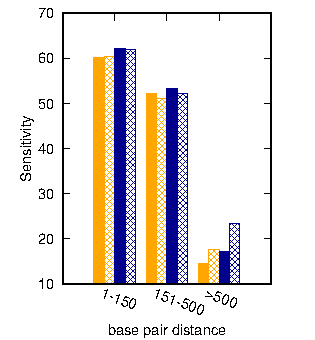
\includegraphics[width=0.35\textwidth]{figs/bylen_bar_recall_hzhang} \\
\hspace{-6.cm} \panel{C} & \hspace{-6cm}\panel{D} \\[-0.5cm]
\hspace{-0.35cm}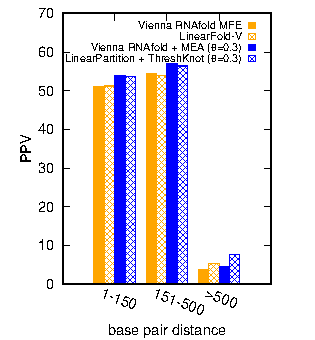
\includegraphics[width=0.35\textwidth]{figs/bylen_bar_precision_hzhang_threshknot} &
\hspace{-0.35cm}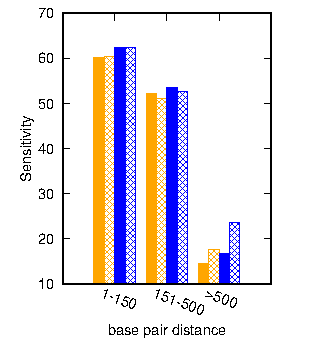
\includegraphics[width=0.35\textwidth]{figs/bylen_bar_recall_hzhang_threshknot}
\end{tabular}
  \caption[.]{Accuracy comparison of base pair prediction with different base pair distances. 
  Each bar represents the overall PPV/sensitivity of all predicted 
base pairs in a certain length range across all sequences. 
\linearpartition performs best on long base pairs over four systems. 
{\bf A} and {\bf B}: Comparison using MEA structures. 
{\bf C} and {\bf D}: Comparison using \threshknot structures.
In all cases, \linearpartition's base pair probabilities lead to substantially better accuracies on long-distance pairs (500+ \nts apart).
  \label{fig:distance}}
%\vspace{1cm}
\end{figure}


\iftrue
\begin{figure}[h]
  \centering
%\hspace{-0.5cm}
\begin{tabular}{ll}
{\large\sf A} & {\large\sf B}\\
    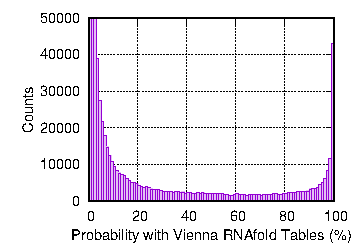
\includegraphics[width=.45\textwidth]{figs/overall_vienna_prob_bin_count}
    &
    \hspace{-0.1cm}
    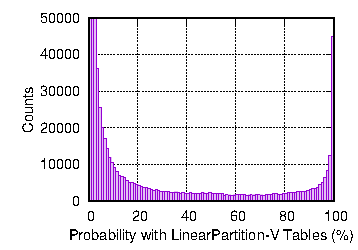
\includegraphics[width=.45\textwidth]{figs/overall_lpv_prob_bin_count}
  \end{tabular} 
  \caption{Pair probability distributions of \viennarnafold and \linearpartitionv are similar.
  {\bf A}: 
  Pair probability distribution of \viennarnafold;
  {\bf B}: 
  Pair probability distribution of \linearpartitionv.
  The count of \linearpartitionv in bin [99,100) is slightly bigger than \viennarnafold, 
  while the count in bin [0,1) (cut here at 50,000) is much less than \viennarnafold 
  (2,068,758 for \linearpartitionv and 48,382,357 for \viennarnafold).
  % This comparison also confirm that \linearpartition prune out lots of base pairs with probabilities close to 0, and the base pairing probability distribution of \linearpartition is peakier.
  \label{fig:bin_counts}}
%\vspace{1cm}
\end{figure}
\fi

% \vspace{-0.6cm}
% \section*{References}
% \balance
% % \bibliographystyle{elsarticle-harv} % can't use any; already used unsrt in pnas-new.cls
% \bibliography{si}




